%!TeX spellcheck = fr-FR
\documentclass[10pt,fleqn]{article} % Default font size and left-justified equations
\usepackage[%
    pdftitle={SLCI : Transformée de Laplace},
    pdfauthor={Xavier Pessoles}]{hyperref}

\usepackage{import}
\usepackage{subcaption}
\subimport{../../../../style/}{preambule.tex}
%\fichetrue
\fichefalse
\proftrue
%\proffalse
%\tdtrue
\tdfalse
\courstrue
%\coursfalse
\subimport{../../../../style/}{new_style}
\subimport{../../../../style/}{macros_SII}
\subimport{../../../../style/}{preambule_trou.tex}

\usepackage{siunitx}
% -------------------------------------
% Déclaration des titres
% -------------------------------------

\def\discipline{Enseignement \\Technologique \\ Transversal}
\def\xxtete{Enseignement Technologique Transversal}

\def\classe{1 STI2D}
\def\xxnumpartie{Seq 3}
\def\xxpartie{Alimenter un système en énergie}

\def\xxnumchapitre{Séance 3}
\def\xxchapitre{\hspace{.12cm} Distribuer l'énergie}

\def\xxposongletx{2}
\def\xxposonglettext{1.45}
\def\xxposonglety{23}
\def\xxonglet{Seq. 3 -- Se. 3}

\def\xxactivite{Cours}
\def\xxauteur{\textsl{Geoffrey Vaquette}}

\def\xxcompetences{%
\textsl{%
\textbf{Savoirs et compétences :}
\begin{itemize}[label=\ding{112},font=\color{ocre}]
\item CO2.1	Identifier les flux et la forme de l'énergie, caractériser ses transformations et/ou modulations et estimer l'efficacité globale d'un système.
\end{itemize}
%
}}

\def\xxfigures{
\begin{center}
% 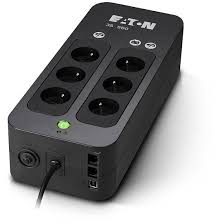
\includegraphics[width=2cm]{images/onduleur} \\
% 
\includegraphics[width=2cm]{images/robinet} \\
%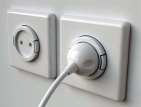
\includegraphics[width=2cm]{images/prise.png} \\
\end{center}
}%figues de la page de garde
\def\xxpied{%
La fonction alimenter/stocker \xxactivite%
}

%---------------------------------------------------------------------------

\renewcommand{\RemplirTrou}{false}
\begin{document}
\chapterimage{images/bandeau}
\subimport{../../../../style/}{new_pagegarde}

\begin{figure}[h]
  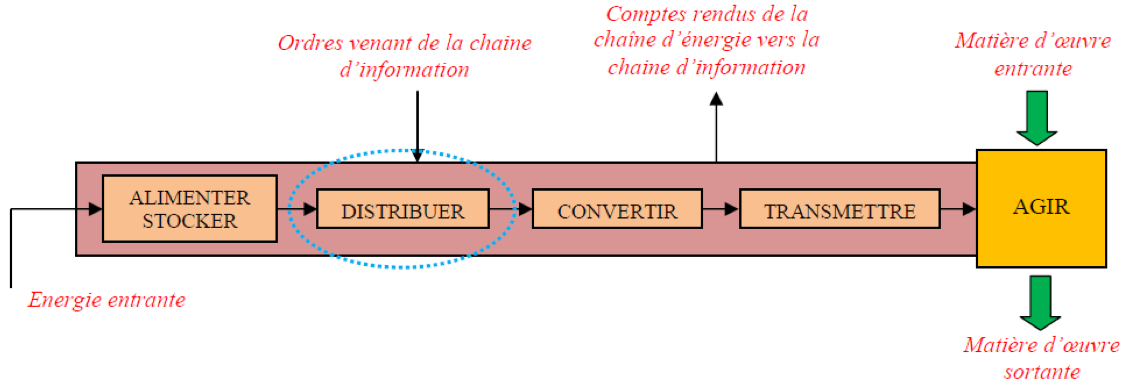
\includegraphics[width=\textwidth]{images/S03_C02}
  \caption{La fonction « Distribuer » dans la chaîne d'énergie}
  \label{fig:chaine}
\end{figure}

Nous avons vu qu'un système ne peut fonctionner que s'il est alimenté en énergie. Une fois l'énergie arrivée jusqu'au système, il faut l'adapter et la distribuer aux différents organes du système.
C'est l'objectif des composants de la fonction distribuer de la chaîne d'énergie.

\section{La fonction « Distribuer »}
\begin{definition}
  La fonction « Distribuer » de la chaîne d'énergie reçoit des ordres de la part de la chaîne d'information et distribue l'énergie dans le système suivant ces ordres.

  L’énergie est de la même forme en entrée et en sortie. La particularité de cette fonction est qu’une faible énergie de commande venant de la chaîne d’information (ordre) doit entraîner le passage ou non d'une énergie dans la suite de la chaîne d'énergie.
\end{definition}


\begin{figure}[h]
  \centering
  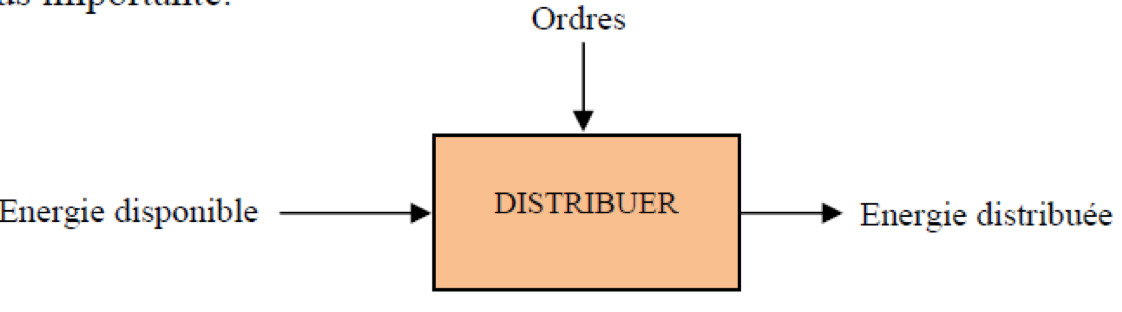
\includegraphics[width=0.6\textwidth]{images/distribuer}
  \caption{La fonction « Distribuer »}
\end{figure}


\begin{exemple}~


  \begin{minipage}{0.7\textwidth}
    Prenons comme exemple un robinet. L’énergie d’entrée du robinet est l’énergie hydraulique (énergie disponible) qui peut être dans les canalisations ou dans un réservoir (le réservoir remplit la fonction « Alimenter / Stocker »).

Lorsque l’homme agit sur le robinet (ordre d’ouverture), l’énergie hydraulique est distribuée et elle est toujours de nature hydraulique.
  \end{minipage}\hfill
  \begin{minipage}{0.2\textwidth}
    
\includegraphics[width=\textwidth]{images/robinet}
  \end{minipage}
\end{exemple}

\section{Les solutions technologiques}

La fonction « Distribuer » est réalisée par des composants appelés « pré-actionneurs »
Le type de pré-actionneur est fonction de la forme et du type d’énergie qu’ils doivent distribuer (électrique, pneumatique, mécanique…)


\subsection{Le relais électromécanique}
Un relais est un composant électromagnétique permettant l’ouverture ou la fermeture d’interrupteurs électriques par un signal de commande.


\begin{figure}[h]
  \begin{subfigure}[b]{.6\textwidth}
    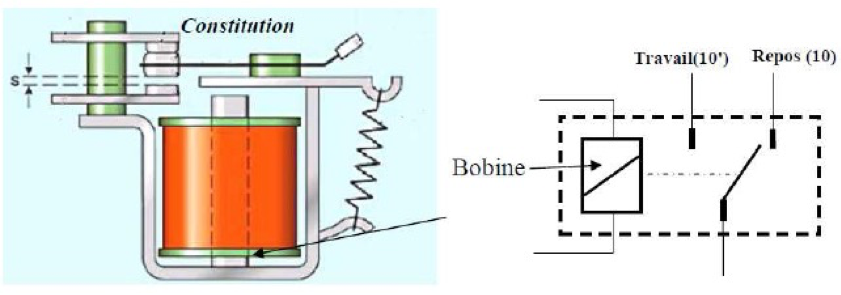
\includegraphics[width=\textwidth]{images/relais_schema}
    \caption{Schéma de principe et schéma électrique d'un relais}
  \end{subfigure}
\hfill
  \begin{subfigure}[b]{.2\textwidth}
    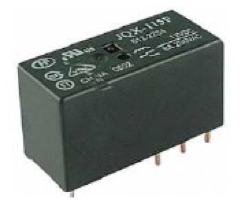
\includegraphics[width=\textwidth]{images/relais_image}
    \caption{Photo d'un relais électro-mécanique}
  \end{subfigure}
  \label{fig:relais}
\end{figure}

Pour faire commuter les contacts du relais, il faut appliquer une tension aux bornes de la bobine, ce qui va créer un courant qui lui-même créera un champ magnétique. Ce dernier fera se déplacer un élément mécanique métallique monté sur un axe mobile, qui déplacera alors des contacts mécaniques.

\paragraph{Les relais bi-stable et mono-stable}
Il existe différents types de relais :
\begin{description}
  \item [Mono-stable : ] les contacts commutent quand la bobine est alimentée et le retour à l'état initial se fait quand la bobine n'est plus alimentée. \textbf{Seul l'état initial est stable car en l'absence de courant, le relais se met automatiquement dans cet état}

  \item [Bi-stable : ] il faut alimenter la bobine pour que les contacts commutent : l'état ne change pas quand la bobine n'est plus alimentée, un système mécanique bloque le retour. Pour revenir à l'état initial, il faut alimenter à nouveau la bobine pour débloquer le mécanisme en inversant la polarité de l'alimentation : exemple télérupteur. \textbf{Les deux états sont stables car ils sont maintenus en l'absence d'ordre.}
\end{description}

\subsection{Le contacteur}
Il fonctionne sur le même principe que le relais mais il est principalement utilisé en électrotechnique lorsque de très fortes puissances sont à commuter.
\begin{figure}[h]
  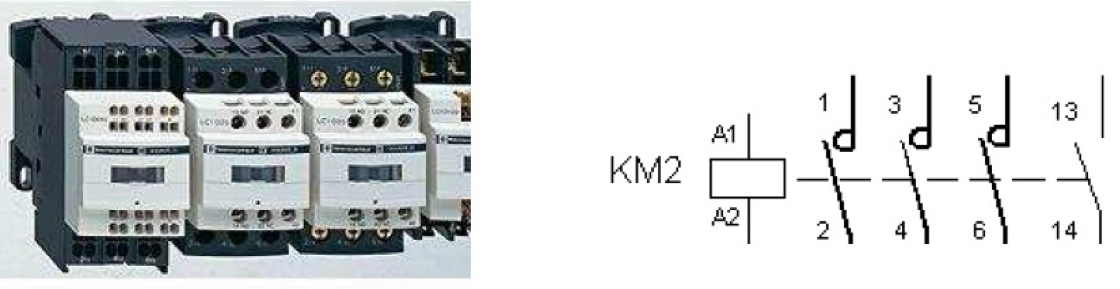
\includegraphics[width=\textwidth]{images/contacteur}
  \caption{Le contacteur électrique}
  \label{fig:contacteur}
\end{figure}
\subsection{Les transistors}

Sur des circuit électronique, la fonction distribuer est remplie par des composants beaucoup plus petits : les transistors.
\subsubsection{Les transistors bipolaires}

\begin{figure}[h]
  \centering
  \begin{subfigure}{0.5\textwidth}
    \centering
    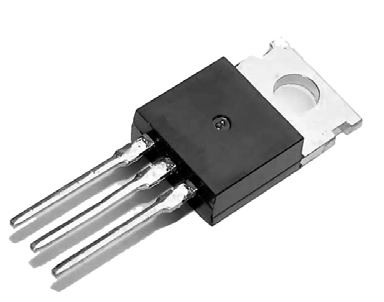
\includegraphics[width=0.5\textwidth]{images/transistor_img}
    \caption{Un transistor bipolaire}
  \end{subfigure}\hfill
  \begin{subfigure}{.5\textwidth}
    \centering
    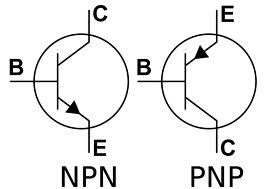
\includegraphics[width=0.5\textwidth]{images/npn_pnp}
    \caption{Symbole électrique d'un transistor}
  \end{subfigure}
  \caption{Transistor bipolaire}
  \label{fig:transistor}
\end{figure}

Un transistor bipolaire est un dispositif électronique à base de semi-conducteur de la famille des transistors.
Son principe de fonctionnement est basé sur deux jonctions PN, l'une en direct et l'autre en inverse.
Il permet de « commander » un courant important à partir d'un courant faible, suivant le principe de l'amplification de courant.

Un transistor bipolaire peut être utilisé en commutation ou en amplification. Nous nous intéressons ici au comportement en commutation

\begin{aretenir}
  Un transistor comporte trois connexions : L'émetteur (E), la base (B) et le collecteur (C).
\end{aretenir}

\begin{remark}
  L'émetteur est \textbf{toujours} associé à une flèche qui indique le sens du courant dans la jonction entre la base et l'émetteur.
\end{remark}

\begin{figure}[h]
  \centering
  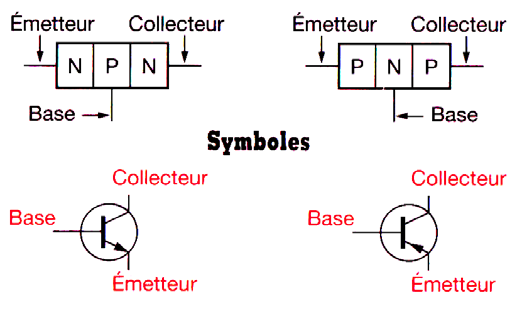
\includegraphics[width=0.4\textwidth]{images/schema_transistor}
  \caption{Deux types de transistor différents}
  \label{fig:npn_pnp}
\end{figure}

\subsubsection{Principe de fonctionnement et règles à retenir}
% \begin{figure}
%   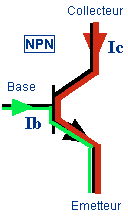
\includegraphics[width=.2\textwidth]{images/principe_transistor}
%   \caption{Principe de fonctionnement d'un transistor}
%   \label{fig:principe}
% \end{figure}

\begin{aretenir}~\\
  \begin{minipage}{.8\textwidth}
    Un transistor fonctionne comme un amplificateur de courant : Un petit courant $I_B$circulant dans la \textbf{base} du transistor induit un courant $I_C$ \textbf{beaucoup plus important du collecteur vers l'émetteur}. Plus précisément, le courant de base est multiplié par un coefficient $\beta$ :
    $$I_C = \beta I_C$$
  \end{minipage}
  \begin{minipage}{.15\textwidth}
    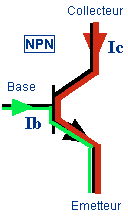
\includegraphics[width=\textwidth]{images/principe_transistor}
  \end{minipage}
\end{aretenir}

\begin{exemple}~\\
  \begin{minipage}{.6\textwidth}
    Dans le cas d'un transistor avec un coefficient $\beta=\num{200}$, on a un courant \num{200} fois plus important dans le collecteur que dans la base. Dans la figure ci-contre, on a $I_C = \beta I_B = 200 \times \num{0.005} = \SI{1}{A}$.
  \end{minipage}
  \begin{minipage}{.35\textwidth}
    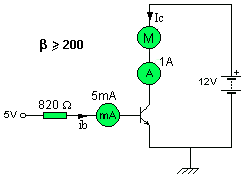
\includegraphics[width=\textwidth]{images/exemple_moteur}
  \end{minipage}
\end{exemple}


\begin{remark}
  Le coefficient $\beta$ est souvent noté \textbf{Hfe} dans les catalogues constructeurs. Il est parfois aussi appelé coefficient d'amplification statique en courant. En général : $30 < \beta < 300$
\end{remark}

  Comme on peut le voir dans l'exemple précédent, deux sources d'alimentation sont nécessaires pour assurer le fonctionnement d'un transistor :
  \begin{description}
    \item[Alimentation du circuit Base : ] Souvent noté $V_{BB}$
    \item[Alementation du circuit Collecteur :] Souvent noté $V_{CC}$
  \end{description}

\subsubsection{Fonctionnement en communtation}
  Lorsque le transistor fonctionne en commutation, il se comporte comme un relais statique (comme un interrupteur) : \textbf{Si $V_{be} = 0$ le courant ne passe pas, si $V_{be}>0.7$ le courant passe}.

  \begin{figure}[h]
    \begin{subfigure}{.45\textwidth}
      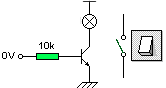
\includegraphics[width=.6\textwidth]{images/transistor_ouvert}
      \centering
      \caption{Le courant de base est nul $\Rightarrow$ le transistor est \textbf{bloqué}. C'est équivalent à un interrupteur \textbf{ouvert}.}
    \end{subfigure}\hfill
    \begin{subfigure}{.45\textwidth}
      \centering
      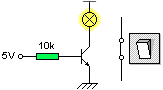
\includegraphics[width=.6\textwidth]{images/transistor_ferme}
      \caption{Le courant de base est suffisant $\Rightarrow$ le transistor est \textbf{saturé}. C'est équivalent à un interrupteur \textbf{fermé}.}
    \end{subfigure}

    \caption{En commutation le transistor est soit \textbf{bloqué} soit \textbf{saturé}}
    \label{}
  \end{figure}

\subsubsection{Les transistors MOS}
  Il existe également des transistor MOS. Ils se comportent également comme des interrupteurs electroniques. Ils sont composés d'une \textbf{source}, d'un \textbf{drain} et d'une \textbf{grille}. C'est la tension $V_{gs}$ entre la grille et la source qui détermine l'état du transistor.

  \begin{remark}
    Ce type de transistor permet de commander un fort courant sans consommation d'énergie. Ils sont souvent utilisés pour commander des moteurs à courant continu.
  \end{remark}

  \begin{aretenir}
    \textbf{$V_{gs} =0 \Rightarrow$ Transitor bloqué,\hfill $V_{gs} >0 \Rightarrow$ Transitor saturé (passant).}
  \end{aretenir}

  \begin{figure}[h]
    \centering
    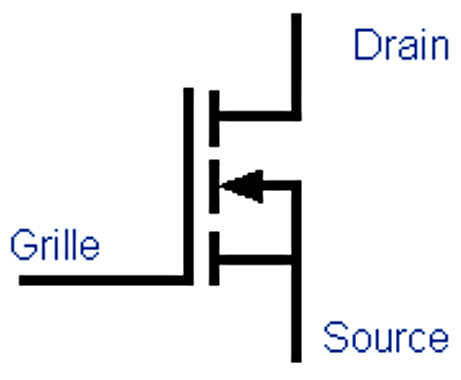
\includegraphics[width=.2\textwidth]{images/mos}
    \caption{Un transistor MOS}
    \label{}
  \end{figure}

\section{Convertisseurs statiques}
  Un convertisseur statique est un système permettant d'adapter la source d'énergie électrique à un récepteur donné en la convertissant.
  Les premiers convertisseurs de puissance électrique ont été réalisés avec des machines électriques couplées mécaniquement.
  Avec l'apparition des semi-conducteurs et de l'électronique de puissance,
  les systèmes de conversion deviennent de plus en plus éllaborés et ne nécessitent plus de machines tournantes. C'est l'ère des convertisseurs statiques.


  \paragraph{}
  Le tableau~\ref{tab:convertisseur} répertorie quelques types de convertisseurs statiques existants. Nous ne décrirons dans ce cours que le transformateur électrique parfait. Les hacheurs pourront être étudiés lors d'un futur TD.

  \begin{table}[h]
    \centering
    \begin{tabular}{c|c|c|c}
      \textbf{Type de convertisseur} & \textbf{Energie en entrée}&\textbf{Energie en sortie} &\textbf{Réglage puissance }\\\hline \hline
      Hacheur                 & Courant continu     & Courant continu     & Oui \\\hline
      Onduleur               & Courant continu     & Courant alternatif  & Oui \\\hline
      Redresseur à diode      & Courant alternatif  & Courant continu     & Non \\\hline
      Transformateur parfait  & Courant alternatif  & Courant alternatif  & Non \\
    \end{tabular}
    \caption{Quelques convertisseurs de puissance}
    \label{tab:convertisseur}

  \end{table}

\subsection{Le transformateur électrique parfait}
\begin{figure}
  \centering
  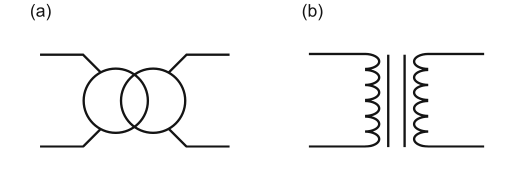
\includegraphics{images/Symb-transfo}
  \caption{Symbole électrique d'un transformateur électrique}
  \label{fig:symb_transfo}
\end{figure}
Un transformateur est un composant permettant d'adapter (augmenter ou abaisser) une tension sinusoïdale. Il est composé de deux bobines de cuivre (inductances) autour d'un circuit magnétique.

La circulation de courant au sein d'une bobine (la bobine primaire) induit un champ magnétique dans le circuit magnétique. Ce champ magnétique induit à son tour un courant électrique dans le circuit secondaire.

\begin{figure}[h]
  \centering
  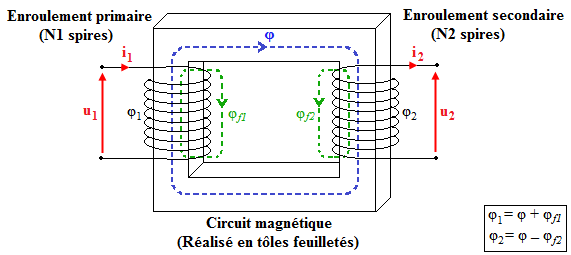
\includegraphics[width=.6\textwidth]{images/transfo_principe}
  \caption{Principe de fonctionnement d'un transformateur}
  \label{fig:principe}
\end{figure}


\begin{aretenir}
  Le courant et la tension dans le circuit secondaire dépendent directement du courant et de la tension dans le circuit primaire. Plus précisément, le \textbf{rapport transformation} $m$ est tel que :
  \begin{center}
      \fbox{$m = \frac{N_2}{N_1} = \frac{U_1}{U_2} = \frac{I_2}{I_1} $}
  \end{center}
\end{aretenir}

\begin{remark}
  Un transformateur parfait n'a pas de perte énergétique, la puissance en entrée est égale à la puissance en sortie.
\end{remark}

\begin{warn}
  Puisque la puissance est constante, lorsqu'un transformateur augmente la tension, il diminue le courant ! $\frac{U_1}{U_2} = \frac{I_2}{I_1}$
\end{warn}
\pagebreak
\section{Quelques lois d'électricité}
\subsection{Les lois de Kirchhoff}
\subsubsection{La loi des noeuds}
\begin{aretenir}
  La somme des intensités des courants qui entrent par un nœud est égale à la somme des intensités des courants qui sortent du même nœud.
\end{aretenir}

\begin{exemple}
  Sur la Figure~\ref{fig:noeud}, la loi des noeuds nous donne la relation $$i_1+i_2=i_3+i_4$$
\end{exemple}

\begin{figure}[h]
  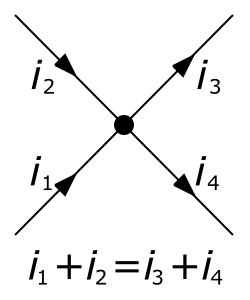
\includegraphics[width=.2\textwidth]{images/loi_des_noeuds}
  \centering
  \caption{Illustration de la loi des noeuds}
  \label{fig:noeud}
\end{figure}

\subsubsection{La loi des mailles}

\begin{aretenir}
  Dans une maille quelconque d'un réseau électrique, la somme algébrique des différences de potentiel le long de la maille est constamment nulle.
\end{aretenir}

\begin{exemple}
  Dans le Figure~\ref{fig:maille}, la loi des mailles nous donne : $$V_1 - V_2 - V_3 - V_4 = 0 \Leftrightarrow V_1 = V_2 + V_3 + V_4$$
\end{exemple}

\begin{figure}[h]
  \centering
  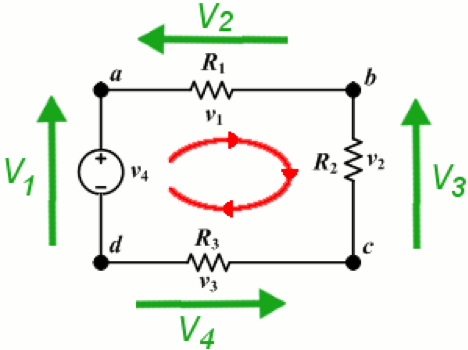
\includegraphics[width=.5\textwidth]{images/loi_des_mailles}
  \caption{Exemple d'application de la loi des mailles}
  \label{fig:maille}
\end{figure}

\subsection{La loi d'Ohm}

\begin{aretenir}
  La loi d'Ohm est une loi physique qui lie l'intensité du courant électrique traversant un dipôle électrique à la tension entre ses bornes et permet de déterminer la valeur d'une résistance.

  Soit $U$ la tension aux borne d'une résistance $R$ et $I$ le courant qui la traverse (cf Figure~\ref{fig:resistance}). La loi d'Ohm s'écrit : $$U = R\dot I$$
\end{aretenir}
\begin{figure}[h]
  \centering
  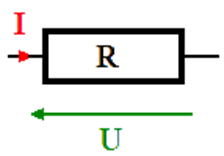
\includegraphics[width=.2\textwidth]{images/resistance}
  \caption{Tension et courant aux borne d'une résistance}
  \label{fig:resistance}
\end{figure}
\end{document}
